% Adaptación de FORMATO.tex para AA3; plantilla original preservada.
\documentclass[12pt,a4paper]{report}

% ------------------------------------------
%   PAQUETES BÁSICOS
% ------------------------------------------
\usepackage[spanish]{babel}
\usepackage[utf8]{inputenc}
\usepackage[T1]{fontenc}
\usepackage{graphicx}
\usepackage{amsmath, amssymb}
\usepackage{booktabs}
\usepackage{geometry}
  \geometry{left=3cm, right=2.5cm, top=3cm, bottom=2.5cm}
\usepackage{setspace}
  \onehalfspacing
\usepackage{titlesec}
  \titleformat{\chapter}[block]{\bfseries\large}{\thechapter.}{1em}{}
  \titleformat{\section}[block]{\bfseries}{\thesection.}{1em}{}
\usepackage{tocloft}
  \setlength{\cftbeforechapskip}{6pt}
  \renewcommand{\cftchapfont}{\bfseries}
\usepackage{longtable}
\usepackage{array}
\usepackage{verbatim}

\usepackage{cite}
\usepackage{hyperref}
% Soporte mínimo para tablas, rutas y bloques técnicos.
\usepackage{calc}
\usepackage{xurl}
\usepackage{fvextra}
\providecommand{\tightlist}{\setlength{\itemsep}{0pt}\setlength{\parskip}{0pt}}
\setlength{\emergencystretch}{3em}

\addto\captionsspanish{
    \renewcommand{\contentsname}{Índice General}
    \renewcommand{\tablename}{Tabla}
}

% ------------------------------------------
%   FONDO DE PÁGINA (SOLO CARÁTULA)
% ------------------------------------------
\usepackage{eso-pic}
\newcommand\BackgroundPic{%
  \put(0,0){%
    \parbox[b][\paperheight]{\paperwidth}{%
      \vfill
      \centering
      \IfFileExists{fondo.jpeg}{\includegraphics[width=\paperwidth,height=\paperheight]{fondo.jpeg}}{\parbox{0.8\paperwidth}{\centering\small [PENDIENTE: fondo.jpeg original]}}%
      \vfill
}}}

% ------------------------------------------
%   ENCABEZADO CON LOGO (OTRAS PÁGINAS)
% ------------------------------------------
\usepackage{fancyhdr}
\pagestyle{fancy}
\fancyhf{}
\setlength{\headheight}{40pt}
\fancyhead[L]{\IfFileExists{logo_unl.jpeg}{\includegraphics[height=1.2cm]{logo_unl.jpeg}}{\fbox{\scriptsize PENDIENTE: logo\_unl.jpeg}}}
\fancyfoot[C]{\thepage}
\renewcommand{\headrulewidth}{0pt}

\fancypagestyle{plain}{
    \fancyhf{}
    \fancyhead[L]{\IfFileExists{logo_unl.jpeg}{\includegraphics[height=1.2cm]{logo_unl.jpeg}}{\fbox{\scriptsize PENDIENTE: logo\_unl.jpeg}}}
    \fancyfoot[C]{\thepage}
    \renewcommand{\headrulewidth}{0pt}
}

% ------------------------------------------
%   METADATOS DEL DOCUMENTO
% ------------------------------------------
\newcommand{\TituloTrabajo}{AA3 -- ADR de alternativas arquitectónicas}
\newcommand{\Autor}{Armas Miguel, Buri Maria, Chamba Richard, Rosillo Odalis}
\newcommand{\Director}{Edison Leonardo Coronel Romero}
\newcommand{\Carrera}{Carrera de Computación}
\newcommand{\Facultad}{Facultad de la Energía, las Industrias y los Recursos Naturales No Renovables}
\newcommand{\Universidad}{Universidad Nacional de Loja}
\newcommand{\Ciudad}{Loja, Ecuador}
\newcommand{\Fecha}{%
  \textnormal{%
    \shortstack{
      \textbf{Semana 3} \\
      12 de octubre de 2026 \\
      18 de octubre de 2026
    }%
  }%
}

\begin{document}

\AddToShipoutPictureBG*{\BackgroundPic}

% ------------------------------------------
%   PORTADA
% ------------------------------------------
\begin{titlepage}
  \centering
  \vspace*{2cm}
  {\bfseries\Large \Universidad}\\[0.5cm]
  {\bfseries\large \Facultad}\\[0.5cm]
  {\bfseries\large \Carrera}\\[2cm]
  {\bfseries\Large \TituloTrabajo}\\[2.5cm]

  \begin{flushright}
    \setlength{\fboxsep}{8pt}
    \fbox{%
      \begin{minipage}{0.4\textwidth}\small
        Desarrollo Basado en Plataformas.
      \end{minipage}%
    }
  \end{flushright}
  \vspace{1cm}

  {\bfseries \large AUTOR:}\\[0.5em]
  {\large \Autor}\\[2em]
  {\bfseries \large TUTOR:}\\[0.5em]
  {\large \Director}\\[2em]
  {\bfseries \large \Ciudad}\\[1em]
  {\bfseries \large \Fecha}
\end{titlepage}

% ------------------------------------------
%   DECLARACIÓN DE USO DE IA GENERATIVA
% ------------------------------------------
\newpage
\chapter*{Declaración de Delegación a IA Generativa}
\addcontentsline{toc}{chapter}{Declaración de uso de IA Generativa}
Se utilizó ChatGPT/Codex para inspeccionar fuentes del proyecto, consultar documentación oficial, comparar alternativas y elaborar el ADR, la matriz y este informe. No se implementó la alternativa ni se ejecutaron nuevas pruebas HTTP o de negocio. La revisión personal y la aceptación humana siguen pendientes.

\noindent\textbf{Declaración enviada por: Armas Miguel, Buri Maria, Chamba Richard, Flores Emilio, Rosillo Odalis.}
\newpage
\clearpage

\chapter{1. Contexto arquitectónico y pregunta de
decisión}\label{analisis-1-contexto-arquitectuxf3nico-y-pregunta-de-decisiuxf3n}

El proyecto organiza autoevaluaciones de carreras con catálogo, modelos
identificables, permisos y trazabilidad. El recorte de Unidad 1
utilizado en APE2/AA2 comprende acceso, catálogo y preparación/consulta
de procesos. ACD3 describe los procesos F-ACD3-01/02 y la arquitectura;
APE3 aporta contratos y verificación parcial de la implementación Spring
existente.

La API actual devuelve DTO directos y errores Problem Details. La
actividad pide un sobre común \path|success/message/data/errors/meta|.
APE3-002 ya registró esta diferencia como propuesta pendiente, pero no
resolvió \textbf{qué parte del backend será responsable de traducir las
respuestas}. Esta es la decisión específica investigada en AA3; no se
vuelve a decidir el monolito modular aceptado por ADR-0001.

\textbf{Pregunta:} si el equipo/docente confirma la adopción del sobre,
¿cómo ubicar su construcción para conservar reglas de negocio
independientes, cubrir respuestas de seguridad y evitar cambios
implícitos en clientes v1?

No se elige aquí entre Spring y Django ni se promete un backend v2
disponible. La guía APE3 exige DRF, mientras el producto usa Spring
Boot: APE3-001 sigue abierto. El análisis se fundamenta en el framework
actualmente implementado y revisa DRF como contraste de una posible
adaptación, sin presentarlo como instalado o seleccionado
definitivamente por el docente.

\section{Insumos revisados y hechos
comprobables}\label{analisis-insumos-revisados-y-hechos-comprobables}

\textbf{Elemento }: Necesidades, RF/RNF y AC

\textbf{Fuente del proyecto }: Dossier/matriz AA2

\textbf{Aporte / límite }: RF-14, RNF-03/07/09/10, AC-AA-03/26 y
VC-AA-03/07/09/10. No son requisitos nuevos de este AA.

\medskip\hrule\medskip

\textbf{Elemento }: Procesos/decisiones

\textbf{Fuente del proyecto }: Informe ACD3, 2/4/6 y REVISION\_GUIA.md

\textbf{Aporte / límite }: Catálogo, preparación, separación de
responsabilidades y compatibilidad. Decisiones discutidas en una sesión
real no aportadas.

\medskip\hrule\medskip

\textbf{Elemento }: C4 implementado/refinado

\textbf{Fuente del proyecto }: APE3 \path|arquitectura/workspace.dsl|

\textbf{Aporte / límite }: Contenedor \path|sigeac.api|; componentes
acceso, http, catálogo, procesos, dominio, repositorios y auditoría.

\medskip\hrule\medskip

\textbf{Elemento }: Contratos

\textbf{Fuente del proyecto }: APE3 OpenAPI observado/objetivo

\textbf{Aporte / límite }: 14 operaciones seleccionadas; el objetivo
declara no implementación. El sobre no es comportamiento vigente.

\medskip\hrule\medskip

\textbf{Elemento }: Presentación actual

\textbf{Fuente del proyecto }: CareerController, SessionController,
ApiProblemHandler y AccessProblemWriter

\textbf{Aporte / límite }: Éxito/controlador, error MVC y error previo
al controlador se construyen en puntos diferentes.

\medskip\hrule\medskip

\textbf{Elemento }: Consumidor

\textbf{Fuente del proyecto }: AccessApi.rememberCsrf, isApiProblem,
career-catalog.page.ts

\textbf{Aporte / límite }: Se lee csrfToken en raíz, se reconoce Problem
Details y se consumen items del catálogo. Envolver cambia esas rutas de
acceso.

\medskip\hrule\medskip

\textbf{Elemento }: Pruebas previas

\textbf{Fuente del proyecto }: Evidencias APE3

\textbf{Aporte / límite }: 23 tests seleccionados y 22 casos HTTP
finales sobre Spring/SQLite; no prueban la arquitectura C propuesta ni
un sobre futuro. No se reejecutaron en AA3.

\medskip\hrule\medskip

Las rutas completas y localizadores están en \url{FUENTES.md}. La
evidencia del consumidor respalda un riesgo concreto: pasar de
\path|session.csrfToken| a \path|session.data.csrfToken| sin migrar el
cliente impediría conservar el token en el punto que hoy lo espera.

\chapter{2. Alternativas y criterios de
comparación}\label{analisis-2-alternativas-y-criterios-de-comparaciuxf3n}

\section{A --- Construir el sobre en cada
controlador}\label{analisis-a--construir-el-sobre-en-cada-controlador}

Cada operación de presentación construye su respuesta explícitamente,
con los puntos de error y seguridad adaptados por separado. Mantiene
visible qué retorna cada ruta y requiere poco mecanismo transversal. Es
razonable para pocas operaciones estables; con varios módulos obliga a
coordinar reglas de error, metadatos y exclusiones en muchos lugares. No
exige trasladar negocio al controlador: ese sería un mal uso, no una
propiedad inevitable de A.

\section{B --- Envolver transversalmente las respuestas
MVC}\label{analisis-b--envolver-transversalmente-las-respuestas-mvc}

Usar un mecanismo transversal de presentación, por ejemplo
\path|ResponseBodyAdvice|, con reglas de inclusión/exclusión y
tratamiento coordinado de errores/filtros. Reduce llamadas repetidas, a
cambio de hacer menos visible la transformación en cada operación. Es
razonable cuando la superficie JSON y sus excepciones están bien
delimitadas. El advice por sí solo no cubre una respuesta que el filtro
escribe directamente al servlet; B completa debe contemplar ese camino y
probarlo, no ignorarlo.

\section{C --- Adaptadores explícitos de presentación y política
compartida}\label{analisis-c--adaptadores-expluxedcitos-de-presentaciuxf3n-y-poluxedtica-compartida}

Definir un contrato de salida tipado y mapeos explícitos en la frontera
API, con una política compartida para los escritores de éxito/error que
corresponda. El controlador conserva la selección visible de respuesta;
la traducción común se concentra fuera de la aplicación/dominio. Los
errores de seguridad requieren su punto de integración propio. No se
propone un servicio desplegable ni un adaptador de persistencia: son
responsabilidades de presentación dentro del mismo backend.

Se selecciona \textbf{C como propuesta individual}, condicionada a
aceptación real del sobre y una estrategia compatible de
contrato/cliente. Los nombres de futuros tipos o mapeadores no se
atribuyen al código existente. La decisión completa está en
\href{ADR-AA3-001-adaptacion-respuestas-api.md}{ADR-AA3-001}.

\section{Criterios derivados del
contexto}\label{analisis-criterios-derivados-del-contexto}

\textbf{ID }: CR-01

\textbf{Criterio pertinente }: Estabilidad para consumidor y contrato

\textbf{Justificación y forma de contrastarlo }: RNF-10, ADR-0018 y
lecturas reales del cliente; comparar paths JSON, headers y estados de
cada operación antes/después.

\medskip\hrule\medskip

\textbf{ID }: CR-02

\textbf{Criterio pertinente }: Cobertura de respuestas y semántica

\textbf{Justificación y forma de contrastarlo }: RF-14, 26 y
logout AC-AA-03; incluir éxito, DTO inválido, rechazo de seguridad y 204
sin cuerpo.

\medskip\hrule\medskip

\textbf{ID }: CR-03

\textbf{Criterio pertinente }: Separación y mantenibilidad

\textbf{Justificación y forma de contrastarlo }: RNF-09 y reglas
ArchUnit; ningún formato HTTP debe entrar en aplicación/dominio por esta
decisión.

\medskip\hrule\medskip

\textbf{ID }: CR-04

\textbf{Criterio pertinente }: Testabilidad y trazabilidad

\textbf{Justificación y forma de contrastarlo }: VC-AA-09/10; poder
localizar mapeo, operación, schema y prueba exacta.

\medskip\hrule\medskip

\textbf{ID }: CR-05

\textbf{Criterio pertinente }: Complejidad/coste de evolución

\textbf{Justificación y forma de contrastarlo }: Recorte de un equipo y
módulos existentes; revisar puntos a cambiar y excepciones, sin inventar
horas estimadas.

\medskip\hrule\medskip

\textbf{ID }: CR-06

\textbf{Criterio pertinente }: Dependencia tecnológica/integración

\textbf{Justificación y forma de contrastarlo }: Spring actual y DRF
pendiente; distinguir política de respuesta de hooks específicos del
framework.

\medskip\hrule\medskip

\textbf{ID }: CR-07

\textbf{Criterio pertinente }: Privacidad/correlación

\textbf{Justificación y forma de contrastarlo }: RNF-03/07,26;
comprobar datos que se exponen y correlación, incluyendo errores previos
al controlador.

\medskip\hrule\medskip

No se ponderan números sin acuerdo ni se inventan benchmarks.
Escalabilidad de despliegue, colas o tamaño de base no discriminan
directamente esta decisión: ninguna alternativa crea por sí misma nuevos
procesos ni resuelve disponibilidad. La asignación de prioridades es una
propuesta individual: primero semántica/compatibilidad/separación;
después coste de coordinación. Si cambian estas prioridades, debe
revisarse la conclusión.

\section{Comparación
argumentada}\label{analisis-comparaciuxf3n-argumentada}

\textbf{Alternativa }: A

\textbf{Ventajas para este proyecto }: Resultado explícito por ruta;
reutiliza el estilo actual de ResponseEntity; introduce pocos
mecanismos.

\textbf{Limitaciones y coste }: Repetir selección de campos en varias
API/handlers; coordinar cambios y pruebas en más puntos.

\textbf{Riesgos y tratamiento }: Divergencia de message/errors/meta o
sobre olvidado; mitigar con schemas, helpers acotados y pruebas de
contrato.

\medskip\hrule\medskip

\textbf{Alternativa }: B

\textbf{Ventajas para este proyecto }: Un punto transversal puede
aplicar política a muchas respuestas MVC; menos invocaciones visibles
por controlador.

\textbf{Limitaciones y coste }: Requiere seleccionar métodos/conversores
y exclusiones; writers de filtro necesitan integración adicional.

\textbf{Riesgos y tratamiento }: Doble envoltura, media type incorrecto
o modificación de 204/archivos; mitigar con opt-in, exclusiones
explícitas y pruebas de todas las salidas.

\medskip\hrule\medskip

\textbf{Alternativa }: C

\textbf{Ventajas para este proyecto }: Mapeo explícito y compartido,
trazable a cada contrato; conserva negocio fuera de HTTP; puntos de
seguridad identificados.

\textbf{Limitaciones y coste }: Añade tipos/mapeos y coordinación; no
elimina todas las llamadas ni asegura consistencia automáticamente.

\textbf{Riesgos y tratamiento }: Sobreingeniería o política duplicada
entre writers; mitigar con pocos tipos necesarios, política única
revisada y pruebas conjuntas.

\medskip\hrule\medskip

Las afirmaciones sobre ventajas/costes son \textbf{inferencias de
diseño} desde el código y los puntos de extensión documentados, no
resultados de prototipos comparativos. Spring documenta respuesta HTTP y
advice ; el código confirma el writer fuera de MVC. DRF muestra también un punto de manejo de excepciones de
vistas cuyo alcance debe distinguirse de respuestas directas.
No se afirma que A o B incumplan necesariamente requisitos: pueden
cumplirlos con disciplina y controles.

\section{Respuesta de cada alternativa a los
requisitos}\label{analisis-respuesta-de-cada-alternativa-a-los-requisitos}

\textbf{Requisito / restricción }: RF-14 / 26: error estable y
seguro

\textbf{A }: Cada handler/writer implementa política; comprobar ausencia
de divergencia.

\textbf{B }: Advice ayuda en MVC; coordinar handlers y writers externos.

\textbf{C }: Mapeo/política explícitos en cada frontera; comprobar
integración.

\medskip\hrule\medskip

\textbf{Requisito / restricción }: RNF-03/07: privacidad y
correlación

\textbf{A }: Selección de datos en cada punto; riesgo de omisión.

\textbf{B }: Política central para lo interceptado; salida de filtro
debe incluirse.

\textbf{C }: Datos públicos/correlación definidos por contrato y
escritores coordinados; revisar lista permitida.

\medskip\hrule\medskip

\textbf{Requisito / restricción }: RNF-09: reglas separadas

\textbf{A }: Cumple si solo presenta resultados y no mueve reglas.

\textbf{B }: Cumple si limita advice a transporte.

\textbf{C }: Cumple si adaptadores permanecen en presentación y no
filtran HTTP hacia aplicación.

\medskip\hrule\medskip

\textbf{Requisito / restricción }: RNF-10: contrato verificable

\textbf{A }: Schema por operación; validación repetida.

\textbf{B }: Debe describir resultado transformado, no solo tipo del
controlador.

\textbf{C }: Contrato explícito de salida y prueba por mapeo/operación.

\medskip\hrule\medskip

\textbf{Requisito / restricción }: ADR-0018 / consumidor actual

\textbf{A }: No migrar silenciosamente v1.

\textbf{B }: La envoltura global también rompe v1 si cambia cuerpos sin
acuerdo.

\textbf{C }: Migración coordinada por superficie/versión a definir; C no
evita ruptura por sí sola.

\medskip\hrule\medskip

\textbf{Requisito / restricción }: Recorte viable / mantenimiento

\textbf{A }: Menor arranque, mayor repetición al crecer.

\textbf{B }: Menor repetición aparente, mayor complejidad de
reglas/excepciones.

\textbf{C }: Coste inicial de diseño, cambio localizado y visible;
justificar solo tipos necesarios.

\medskip\hrule\medskip

\textbf{Requisito / restricción }: Tecnología APE3 pendiente

\textbf{A }: Se puede trasladar el principio a DRF, con APIs distintas.

\textbf{B }: El hook ResponseBodyAdvice no es portable directamente a
DRF.

\textbf{C }: Política/mapeos conceptuales portables; integración
concreta sí depende del framework.

\medskip\hrule\medskip

\chapter{3. Responsabilidades, decisión y verificación
futura}\label{analisis-3-responsabilidades-decisiuxf3n-y-verificaciuxf3n-futura}

\section{Organización propuesta y correspondencia C4}
\label{sec:organizacion_c4}

\begin{figure}[htbp]
    \centering
    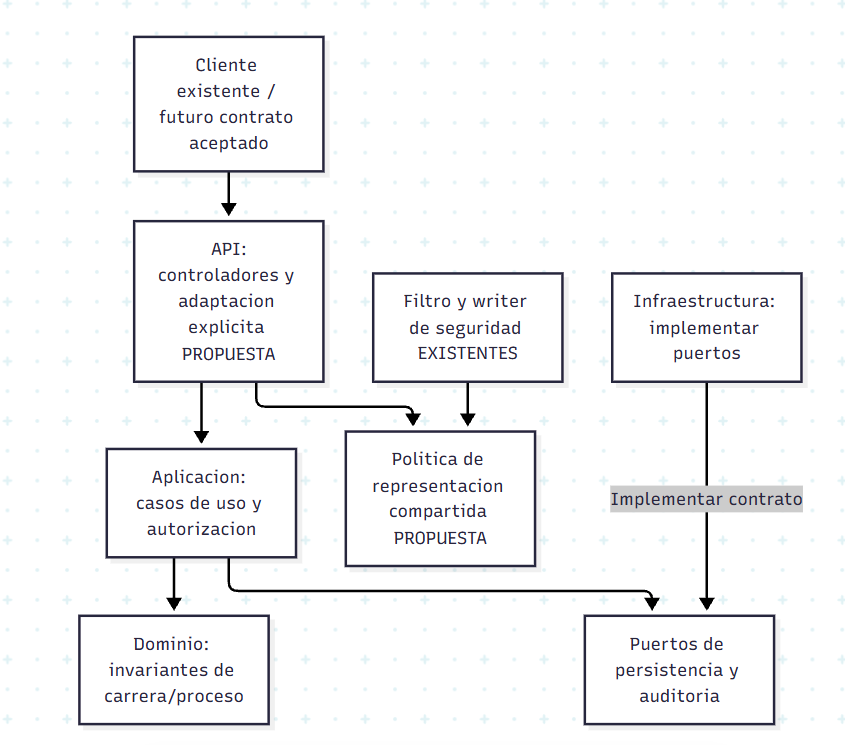
\includegraphics[width=0.85\textwidth]{Diagrama1.png}
    \caption{Organización propuesta y correspondencia C4.}
    \label{fig:organizacion_c4}
\end{figure}
Las flechas continuas expresan uso; la discontinua, implementación del
puerto. El diagrama combina responsabilidades existentes y propuestas,
etiquetadas; no es una vista de despliegue nueva. No afirma que todos
los DTO actuales sean resultados de aplicación independientes: esa
separación debe comprobarse por operación antes de adaptar.

En C1 no cambian actores ni sistemas externos. En C2 se conserva el
backend único; no se añade un gateway o microservicio. En C3 la
propuesta corresponde a \path|sigeac.api.http| y al borde escritor de
\path|sigeac.api.acceso|; catálogo/procesos/dominio/repositorios
mantienen sus funciones. Los detalles de un futuro mapeador serían
elementos de código, no contenedores C4.

\textbf{Parte }: API/presentación

\textbf{Responsabilidad }: Validar estructura de entrada, traducir
resultados/errores al contrato, seleccionar HTTP y headers.

\textbf{Dependencia permitida / mezcla a evitar }: Usar aplicación y
política de salida; no decidir vigencia de carrera ni autoridad
institucional.

\medskip\hrule\medskip

\textbf{Parte }: Política/mapeos propuestos

\textbf{Responsabilidad }: Definir salida pública y metadatos
permitidos; conservar coherencia con status/media type.

\textbf{Dependencia permitida / mezcla a evitar }: Datos necesarios de
salida; no consultar repositorio ni ejecutar permisos para decorar una
respuesta.

\medskip\hrule\medskip

\textbf{Parte }: Aplicación

\textbf{Responsabilidad }: Orquestar caso, permisos, transacción y
puertos.

\textbf{Dependencia permitida / mezcla a evitar }: Dominio/puertos; no
retornar el sobre por mandato de esta propuesta ni depender de tipos
servlet.

\medskip\hrule\medskip

\textbf{Parte }: Dominio

\textbf{Responsabilidad }: Conservar invariantes/estados/revisiones.

\textbf{Dependencia permitida / mezcla a evitar }: No construir JSON,
response entities ni message de UI.

\medskip\hrule\medskip

\textbf{Parte }: Infraestructura

\textbf{Responsabilidad }: Implementar persistencia/adaptadores;
escribir errores de seguridad donde corresponda actualmente.

\textbf{Dependencia permitida / mezcla a evitar }: Respetar puertos y
política de frontera; no asumir permisos por acceso DB. El filtro
escritor es un detalle actual de identidad, no persistencia.

\medskip\hrule\medskip

\section{Plan de comprobación propuesto, no
ejecutado}\label{analisis-plan-de-comprobaciuxf3n-propuesto-no-ejecutado}

PF-AA3-01: al aprobar la política, comparar schemas de cada operación
incluida con cuerpos reales, código HTTP, Content-Type,
Location/ETag/Set-Cookie cuando correspondan. PF-AA3-02: probar errores
de DTO, negocio y filtro, código público/correlación y ausencia de
secretos. PF-AA3-03: verificar logout 204 con cero bytes y exclusiones
de cuerpo aplicables. PF-AA3-04: mantener funcionamiento del consumidor
del contrato conservado y probar cliente migrado. PF-AA3-05: ejecutar
reglas de arquitectura y revisión de imports/SQL pertinentes.

No se crean tests vacíos ni se ejecutan pruebas de la alternativa C que
todavía no existe. La \href{TRAZABILIDAD_ADR.md}{matriz} separa
evidencia existente y verificaciones futuras.

\section{Cierre académico y
pendientes}\label{analisis-cierre-acaduxe9mico-y-pendientes}

\textbf{Actividad AA3 }: 1. Contexto

\textbf{Evidencia preparada }: Sección 1 y fuentes P-01--09.

\medskip\hrule\medskip

\textbf{Actividad AA3 }: 2. Alternativas

\textbf{Evidencia preparada }: A, B y C en sección 2.

\medskip\hrule\medskip

\textbf{Actividad AA3 }: 3. Criterios

\textbf{Evidencia preparada }: CR-01--07, derivados de
requisitos/restricciones.

\medskip\hrule\medskip

\textbf{Actividad AA3 }: 4. Comparación

\textbf{Evidencia preparada }: Ventajas, limitaciones, riesgos y
respuesta por requisito.

\medskip\hrule\medskip

\textbf{Actividad AA3 }: 5. Fuentes oficiales

\textbf{Evidencia preparada }: S-01--08 en FUENTES.md, con localizadores
y límites de versión.

\medskip\hrule\medskip

\textbf{Actividad AA3 }: 6. Respuesta a requisitos

\textbf{Evidencia preparada }: Tabla de alternativas y matriz de
trazabilidad.

\medskip\hrule\medskip

\textbf{Actividad AA3 }: 7. Responsabilidades

\textbf{Evidencia preparada }: Diagrama y tabla C1/C2/C3.

\medskip\hrule\medskip

\textbf{Actividad AA3 }: 8. ADR

\textbf{Evidencia preparada }: ADR-AA3-001: propuesto, selección C y
consecuencias/mitigaciones.

\medskip\hrule\medskip

\textbf{Actividad AA3 }: 9. Relación con proyecto

\textbf{Evidencia preparada }: TRAZABILIDAD\_ADR.md con requisitos,
riesgos, C4, módulos, contrato y pruebas.

\medskip\hrule\medskip



\clearpage
\appendix
\chapter{ADR-AA3-001 --- Adaptación explícita de respuestas en la frontera API}


\section{Contexto}\label{adr-contexto}

AA-RF-14 exige rechazos estables y seguros, AC-RF-26 identifica
código/descripción/correlación; ARNF-03/07/09/10 respaldan privacidad,
diagnóstico, separación y coherencia contractual. Se relacionan con
RF-05 y los actores autorizados RF-01--04. El requisito de sobre
\path|success/message/data/errors/meta| procede de la guía académica, no
de una decisión de producto ya aprobada. Debe resolverse esa aceptación
antes de cambiar la API.

El producto actual es un monolito modular Spring; los controladores
retornan representaciones directas, handlers retornan ProblemDetail y
AccessProblemWriter escribe JSON desde la infraestructura de identidad.
Los clientes consumen \path|session.csrfToken|, \path|CatalogPage.items|
y campos de Problem Details. Una envoltura cambia esas expectativas.
ADR-0018 impide reemplazar silenciosamente DTO v1; el objetivo v2
existente de 005 tiene otros compromisos, no está libre para adjudicarle
este cambio automáticamente.

APE3-002 identifica la incompatibilidad pero deja abierta la
organización interna que produciría el sobre. Debe analizarse antes de
repartir construcción de JSON entre negocio y transporte o activar una
envoltura transversal. Las 22 respuestas comprobadas en APE3 sirven de
línea base del formato actual, no demuestran una alternativa aún no
implementada.


\section{Alternativas consideradas}\label{adr-alternativas-consideradas}

\textbf{Opción }: A

\textbf{Descripción }: Construir sobre por controlador y adaptar cada
handler/writer.

\textbf{Ventaja }: Salida visible, pocas piezas nuevas; razonable con
pocas operaciones.

\textbf{Limitación/riesgo }: Coordinación distribuida y posible
divergencia de campos/reglas.

\medskip\hrule\medskip

\textbf{Opción }: B

\textbf{Descripción }: Envoltura transversal MVC, por ejemplo
ResponseBodyAdvice, más integración de seguridad/errores.

\textbf{Ventaja }: Centraliza transformaciones interceptables y evita
invocaciones repetidas.

\textbf{Limitación/riesgo }: Exige opt-in/exclusiones, revisar
conversores y caminos fuera de MVC; puede ocultar el contrato real de
una operación.

\medskip\hrule\medskip

\textbf{Opción }: C

\textbf{Descripción }: Adaptadores/mapeos explícitos de presentación y
política común para escritores relevantes.

\textbf{Ventaja }: Mantiene visible la salida y concentra reglas de
representación sin introducirlas en negocio.

\textbf{Limitación/riesgo }: Añade mapeos/tipos y coordinación entre API
y seguridad; puede sobredimensionarse.

\medskip\hrule\medskip

A y B son viables si incorporan todos sus controles. C no se justifica
porque las otras sean imposibles, sino por la necesidad local de hacer
explícita la compatibilidad en varios caminos de salida. La comparación
detallada y CR-01--07 están en el informe AA3.

\section{Decisión}\label{adr-decisiuxf3n}

\textbf{Seleccionar C como propuesta de organización}, condicionada a
que se confirme la adopción del sobre. Ubicar la traducción de
resultados a contrato HTTP en la frontera de presentación, con mapeos
explícitos por representación y política compartida de salida pública.
No construir el sobre en servicios de aplicación, objetos de dominio o
repositorios.

Los handlers y el escritor de seguridad deben aplicar la política
acordada mediante sus propios puntos de integración; no dar por hecho
que un advice MVC procesa toda respuesta servlet. Conservar 204 sin
cuerpo y excluir otros intercambios que no admitan ese JSON. No envolver
automáticamente binarios, streams, documentación o endpoints fuera de la
superficie aprobada.

Aplicar una migración coordinada de contrato y cliente, cuya
versión/frontera debe acordarse. No se elige una nueva URL, se altera
v1, se habilita v2 ni se aprueba el sobre mediante este ADR. Para
paginación, resolver si se mantiene CatalogPage dentro de data o se
trasladan campos a meta: ACD3 y APE3 registraron variantes, todavía no
hay acuerdo único. No combinar ambas duplicando totales.

\section{Justificación}\label{adr-justificaciuxf3n}

CR-01/02 dan prioridad a compatibilidad y salidas correctas: el cliente
y el writer actuales muestran varias fronteras que un cambio debe
cubrir. CR-03/04 favorecen separar formato, localizar mapeos y
relacionarlos con pruebas. C ofrece esa visibilidad sin trasladar reglas
a controladores o aplicación. CR-05 limita el diseño: solo tipos/mapeos
necesarios para operaciones aceptadas, sin motor genérico de
serialización. CR-06 distingue política de hooks del framework; CR-07
exige seleccionar explícitamente campos públicos y correlación.

La documentación oficial de Spring respalda ResponseEntity/ProblemDetail
y los puntos de extensión; no prescribe C como superior. \textbf{La
selección es una inferencia de diseño} basada en requisitos/código y en
la incertidumbre de migración. No se obtuvieron métricas comparativas de
rendimiento, defectos, horas o aprendizaje. No se afirma mejora
automática de seguridad o escalabilidad.

\section{Responsabilidades y
dependencias}\label{adr-responsabilidades-y-dependencias}

API: seleccionar método/estado/headers y mapear entrada/salida.
Aplicación: ejecutar caso, reglas de autorización, transacción y
puertos. Dominio: invariantes/estados. Infraestructura: persistir o
integrar, respetando contratos; el writer de identidad es una frontera
HTTP que debe coordinar la representación sin mezclarse con SQL.

C4: sin cambios a C1/C2. Refinar C3 en \path|sigeac.api.http| y su
relación con la salida de \path|sigeac.api.acceso|, del workspace APE3.
Catálogo, procesos, dominio y repositorios no incorporan el sobre como
obligación interna. Los nombres concretos de clases nuevas se definirán
después; no se documentan como existentes.

\section{Consecuencias}\label{adr-consecuencias}

\textbf{Positivas esperadas:} mapeo público localizable y trazable;
separación entre negocio y representación; pruebas de contrato con
puntos de entrada identificables; una política revisable de
metadatos/errores. Son beneficios previstos, no resultados medidos.

\textbf{Negativas/costes:} trabajo inicial de tipos/mapeos, modificación
coordinada de consumidor y esquemas, revisión de múltiples escritores y
mantenimiento de compatibilidad durante transición. C no evita que un
mapeador mal programado omita campos o filtre secretos. No se justifica
migrar toda la API ni añadir otro servicio por este ADR.

\section{Riesgos y mitigaciones}\label{adr-riesgos-y-mitigaciones}

\textbf{ID }: RK-AA3-01

\textbf{Riesgo concreto }: Cliente v1 deja de leer
csrfToken/items/errores.

\textbf{Mitigación y comprobación futura }: Acordar estrategia de
contrato; conservar pruebas del formato mantenido y ejecutar cliente
migrado. PF-AA3-04.

\medskip\hrule\medskip

\textbf{ID }: RF-AA3-02

\textbf{Riesgo concreto }: Error del filtro queda fuera de política.

\textbf{Mitigación y comprobación futura }: Inventariar writers; probar
rechazo sin sesión y CSRF desde integración completa. PF-AA3-02.

\medskip\hrule\medskip

\textbf{ID }: RK-AA3-03

\textbf{Riesgo concreto }: Se añade cuerpo a 204 o cambian headers.

\textbf{Mitigation y comprobación futura }: \\
Exclusiones y aserciones de bytes/estado/Location/ETag/Set-Cookie por operación. PF-AA3-01/03.

\medskip\hrule\medskip

\textbf{ID }: RK-AA3-04

\textbf{Riesgo concreto }: Mensajes/detalles, exponen secretos o
información ajena.

\textbf{Mitigación y comprobación futura }: Lista de campos públicos,
saneamiento de diagnóstico y marcadores sintéticos; probar
permisos/cuerpos/registros pertinentes. PF-AA3-02.

\medskip\hrule\medskip

\textbf{ID }: RK-AA3-05

\textbf{Riesgo concreto }: Se crean mapeadores genéricos innecesarios o
reglas entran en presentación.

\textbf{Mitigación y comprobación futura }: Limitar superficie; revisar
dependencias y reglas ArchUnit. PF-AA3-05.

\medskip\hrule\medskip

\textbf{ID }: RK-AA3-06

\textbf{Riesgo concreto }: Se aplica un hook/versionado de framework no
confirmado.

\textbf{Mitigación y comprobación futura }: Confirmar Spring/DRF y
versión resuelta antes de implementar; repetir evaluación de
integración.

\medskip\hrule\medskip

\textbf{ID }: RK-AA3-07

\textbf{Riesgo concreto }: OpenAPI, paginación, media type y cuerpo
divergen.

\textbf{Mitigación y comprobación futura }: Acordar un schema aceptado,
validar muestras y mantener pares request/response y casos negativos.
PF-AA3-01/02.

\medskip\hrule\medskip

HTTP-AA-01, 401 sin desafío explícito, sigue abierto: rediseñar el JSON
no lo resuelve. La aceptación del ADR debe contemplar este límite de
RNF-10 sin inventar un esquema Bearer.

\section{Relación con implementación y
pruebas}\label{adr-relaciuxf3n-con-implementaciuxf3n-y-pruebas}

Línea base: SessionController, CareerController, ApiProblemHandler,
CareerCatalogProblemHandler y AccessProblemWriter;
AccessApi.rememberCsrf e isApiProblem del cliente; contratos/evidencias
APE3. Rutas completas en \url{FUENTES.md}.

Ver \url{TRAZABILIDAD_ADR.md}: RF/RNF\ensuremath{\rightarrow}ADR\ensuremath{\rightarrow}componente C4\ensuremath{\rightarrow}implementación
existente o cambio propuesto\ensuremath{\rightarrow}prueba existente o PF futura. No se marca
como verificada una relación con código nuevo inexistente. Las reglas
\path|DOMAIN_IS_INDEPENDENT| y
\path|APPLICATION_IGNORES_API_AND_INFRASTRUCTURE| existen en
ModuleArchitectureTest; no verifican por sí solas el contenido JSON, la
privacidad o los caminos de seguridad.

\chapter{AA3 --- Matriz de trazabilidad del
ADR}\label{traza-aa3--matriz-de-trazabilidad-del-adr}

ADR-AA3-001 está \textbf{Propuesto}, con alternativa C seleccionada para
revisión. P-XX/S-XX remiten a \url{FUENTES.md}. Los PF son
verificaciones futuras, no pruebas ejecutadas ni requisitos oficiales
nuevos.

\textbf{Origen / necesidad }: N-AA-05, comprender rechazo; A-AA-01--04

\textbf{Requisito y criterio }: RF-14; AC-AA-26

\textbf{Riesgo / criterio comparativo }: RF-02/04/07; CR-02/07

\textbf{ADR y componente C4 }: ADR-AA3-001 C; http y acceso

\textbf{Código o contrato identificado }: ApiProblemHandler,
CareerCatalogProblemHandler, AccessProblemWriter; OpenAPI
observado/objetivo

\textbf{Evidencia y estado }: Errores actuales en APE3
HTTP-01/04/05/07/09/11/14/16. PF-AA3-02 pendiente para C.

\medskip\hrule\medskip

\textbf{Origen / necesidad }: N-AA-01/04, privacidad

\textbf{Requisito y criterio }: RNF-03; VC-AA-03

\textbf{Riesgo / criterio comparativo }: RK-04; CR-07

\textbf{ADR y componente C4 }: Política pública propuesta en frontera

\textbf{Código o contrato identificado }: Cuerpos/handlers y ámbitos
existentes; no mapper C implementado

\textbf{Evidencia y estado }: Redacción de evidencia APE3 no demuestra
privacidad completa. Prueba con secretos/ámbitos pendiente.

\medskip\hrule\medskip

\textbf{Origen / necesidad }: N-AA-05, diagnóstico

\textbf{Requisito y criterio }: RNF-07; VC-AA-07

\textbf{Riesgo / criterio comparativo }: RK-02/04; CR-07

\textbf{ADR y componente C4 }: http/acceso y correlación

\textbf{Código o contrato identificado }: CorrelationFilter y
extensiones de error actuales

\textbf{Evidencia y estado }: Muestras incluyen correlationId; relación
completa con logs/éxitos y contrato futuro pendiente.

\medskip\hrule\medskip

\textbf{Origen / necesidad }: N-AA-05, reglas verificables

\textbf{Requisito y criterio }: RNF-09; VC-AA-09

\textbf{Riesgo / criterio comparativo }: RK-05; CR-03/04

\textbf{ADR y componente C4 }: Mantener aplicación/dominio fuera de
sobre

\textbf{Código o contrato identificado :} ModuleArchitectureTest: \texttt{DOMAIN\_IS\_INDEPENDENT}, \texttt{APPLICATION\_IGNORES\_API\_AND\_INFRASTRUCTURE}

\textbf{Evidencia y estado }: APE3 registró ejecución de suite de
arquitectura; no prueba C inexistente. PF-05 pendiente.

\medskip\hrule\medskip

\textbf{Origen / necesidad }: N-04/05, intercambio interpretable

\textbf{Requisito y criterio }: RNF-10; VC-10

\textbf{Riesgo / criterio comparativo }: RK-01/03/07; CR-01/02

\textbf{ADR y componente C4 }: Adaptadores explícitos propuestos

\textbf{Código o contrato identificado }: Dos OpenAPI de APE3, contratos
distintos

\textbf{Evidencia y estado }: 22 muestras conformes al observado; cero
pruebas del sobre objetivo. PF-01 pendiente.

\medskip\hrule\medskip

\textbf{Origen / necesidad }: N-AA-01, terminar acceso

\textbf{Requisito y criterio }: RF-02; AC-03

\textbf{Riesgo / criterio comparativo }: RK-AA3-03; CR-02

\textbf{ADR y componente C4 }: Frontera de sesión preserva respuesta
vacía

\textbf{Código o contrato identificado
}: SessionController.revokeCurrentSession; DELETE sessions

\textbf{Evidencia y estado }: APE3 HTTP-20/21: 204 cero bytes y acceso
posterior rechazado. Regresión futura PF-03.

\medskip\hrule\medskip

\textbf{Origen / necesidad }: Consumidor funcional / compatibilidad

\textbf{Requisito y criterio }: ADR-0018; RNF-10

\textbf{Riesgo / criterio comparativo }: RK-01; CR-01/05

\textbf{ADR y componente C4 }: Cambios coordinados de cliente y API

\textbf{Código o contrato identificado }: AccessApi.rememberCsrf,
SessionView, isApiProblem, catálogo items

\textbf{Evidencia y estado }: Lectura de código, sin nueva ejecución
Angular en AA3. PF-AA3-04 pendiente.

\medskip\hrule\medskip

\textbf{Origen / necesidad }: Exigencia académica de sobre

\textbf{Requisito y criterio }: Guías ACD3/APE3; APE3-002 propuesto

\textbf{Riesgo / criterio comparativo }: RK-06/07; CR-05/06

\textbf{ADR y componente C4 }: Condición de aceptación del ADR

\textbf{Código o contrato identificado }: openapi-objetivo.yaml declara
no implementación

\textbf{Evidencia y estado }: Política de paginación y versión/frontera
pendientes. No declarar aprobado por estar especificado.

\medskip\hrule\medskip

\textbf{Origen / necesidad }: Tecnología y arquitectura existentes

\textbf{Requisito y criterio }: Constitución; ADR-0001/0004/0018;
APE3-001 propuesto

\textbf{Riesgo / criterio comparativo }: RK-AA3-06; CR-03/06

\textbf{ADR y componente C4 }: Backend único; C3 http/acceso

\textbf{Código o contrato identificado }: POM Java21/Boot4.1.1, paquetes
Spring; DSL APE3

\textbf{Evidencia y estado }: DRF exigido en APE3 sigue sin resolución.
Documentación oficial consultada no decide por el equipo.

\medskip\hrule\medskip

\section{Verificaciones
propuestas}\label{traza-verificaciones-propuestas}

\textbf{ID }: PF-01

\textbf{Qué comprobar }: Contrato aceptado, estado, schema, Content-Type
y headers de cada operación incluida

\textbf{Evidencia que deberá producirse }: Prueba de contrato más
capturas redactadas de intercambios, versión y resultado.

\medskip\hrule\medskip

\textbf{ID }: PF-02

\textbf{Qué comprobar }: Errores MVC y seguridad, campos públicos,
privacidad y correlación

\textbf{Evidencia que deberá producirse }: Casos negativos de
integración; lector autorizado/ajeno; diagnóstico sin secretos.

\medskip\hrule\medskip

\textbf{ID }: PF-03

\textbf{Qué comprobar }: 204 sin cuerpo y exclusiones semánticas

\textbf{Evidencia que deberá producirse }: Aserción de cero bytes y
headers, regresión del logout; otros métodos/estados solo si la
superficie los implementa.

\medskip\hrule\medskip

\textbf{ID }: PF-04

\textbf{Qué comprobar }: Cliente conservado y migrado interpretan su
contrato

\textbf{Evidencia que deberá producirse }: Pruebas de login/CSRF,
catálogo/páginas y errores sobre entorno/cliente acordados.

\medskip\hrule\medskip

\textbf{ID }: PF-05

\textbf{Qué comprobar }: Aplicación/dominio sin dependencias de
presentación, reglas de negocio fuera de adaptación

\textbf{Evidencia que deberá producirse }: ArchUnit, revisión de
dependencias y pruebas de reglas pertinentes; registrar límites de SQL y
serialización.

\medskip\hrule\medskip


\chapter{AA3 --- Registro de fuentes y
evidencia}\label{fuentes-aa3--registro-de-fuentes-y-evidencia}

Rutas relativas a la raíz. Las fuentes P describen el proyecto; S
fundamentan mecanismos técnicos y forma del ADR. Las ventajas/costes
comparativos y la selección C son inferencias del análisis, no
recomendaciones explícitas de un fabricante ni resultados
experimentales. No se hicieron entrevistas ni nuevas pruebas de negocio.

\section{Fuentes del proyecto}\label{fuentes-fuentes-del-proyecto}

\textbf{ID }: P-01

\textbf{Archivos exactos / localizadores
}: \path|documentos-academicos/AA2-semana-2/DOSSIER_REQUISITOS_AA2.md|,
tablas RF/RNF y AC/VC;
\path|documentos-academicos/AA2-semana-2/MATRIZ_TRAZABILIDAD.md|

\textbf{Uso y límite }: N-AA-05, AA-RF-14, AA-RNF-03/07/09/10; actores y
criterios. No aprobación institucional.

\medskip\hrule\medskip

\textbf{ID }: P-02

\textbf{Archivos exactos / localizadores
}: \path|documentos-academicos/ACD3-semana-3/ACD3_CLINICA_ARQUITECTURA_API.md|,
2/4/6; \path|CONTRATO_API_INICIAL.md|, §4, y \path|REVISION_GUIA.md|,
bajo la misma carpeta

\textbf{Uso y límite }: Procesos, alternativas de respuesta y
compatibilidad. La propuesta preliminar considera paginación en meta; no
es acuerdo aceptado.

\medskip\hrule\medskip

\textbf{ID }: P-03

\textbf{Archivos exactos / localizadores
}: \path|documentos-academicos/APE3-semana-3/adr/APE3-001-alineacion-tecnologica.md|;
\path|documentos-academicos/APE3-semana-3/adr/APE3-002-contrato-universal.md|

\textbf{Uso y límite }: Diferencias de tecnología y sobre todavía
propuestas; AA3 refina una subdecisión, no reemplaza su estado.

\medskip\hrule\medskip

\textbf{ID }: P-04

\textbf{Archivos exactos / localizadores
}: \path|documentos-academicos/APE3-semana-3/arquitectura/workspace.dsl|,
componentes \path|sigeac.api.http| y \path|sigeac.api.acceso|;
\path|documentos-academicos/ACD3-semana-3/ARQUITECTURA_C4.md|

\textbf{Uso y límite }: Ubicación del cambio propuesto en C3; no nuevo
contenedor.

\medskip\hrule\medskip

\textbf{ID }: P-05

\textbf{Archivos exactos / localizadores
}: \path|documentos-academicos/APE3-semana-3/contratos/openapi-observado.yaml|;
\path|documentos-academicos/APE3-semana-3/contratos/openapi-objetivo.yaml|

\textbf{Uso y límite }: Contrato actual de muestra y objetivo no
implementado. El objetivo mantiene CatalogPage dentro de data; confirmar
variante de paginación antes de adoptar.

\medskip\hrule\medskip

\textbf{ID }: P-06

\textbf{Archivos exactos / localizadores
}: \path|backend/src/main/java/ec/edu/unl/sec/selfassessment/api/CareerController.java|,
retornos ResponseEntity;
\path|backend/src/main/java/ec/edu/unl/sec/identityaccess/api/SessionController.java|,
create/revokeCurrentSession;
\path|backend/src/main/java/ec/edu/unl/sec/shared/api/ApiProblemHandler.java|,
problem/handlers;
\path|backend/src/main/java/ec/edu/unl/sec/selfassessment/api/CareerCatalogProblemHandler.java|;
\path|backend/src/main/java/ec/edu/unl/sec/identityaccess/infrastructure/AccessProblemWriter.java|,
write;
\path|backend/src/main/java/ec/edu/unl/sec/identityaccess/infrastructure/SessionAuthenticationFilter.java|,
doFilterInternal;
\path|backend/src/main/java/ec/edu/unl/sec/shared/infrastructure/CorrelationFilter.java|

\textbf{Uso y límite }: Distintos puntos de salida actuales. El writer
escribe al servlet y no retorna desde un método MVC. No se implementó ni
probó advice/mapeador C nuevo.

\medskip\hrule\medskip

\textbf{ID }: P-07

\textbf{Archivos exactos / localizadores
}: \path|frontend/src/app/features/access/data-access/access-api.service.ts|,
login/rememberCsrf;
\path|frontend/src/app/features/access/data-access/access.models.ts|,
SessionView; \path|frontend/src/app/core/http/problem.ts|, isApiProblem;
\path|frontend/src/app/features/careers/pages/career-catalog.page.ts|,
result.items/history

\textbf{Uso y límite }: Acoplamientos comprobables del cliente a las
representaciones existentes. Lectura de código, sin ejecución Angular en
AA3.

\medskip\hrule\medskip

\textbf{ID }: P-08

\textbf{Archivos exactos / localizadores
}: \path|backend/src/test/java/ec/edu/unl/sec/architecture/ModuleArchitectureTest.java|,
DOMAIN\_IS\_INDEPENDENT y
APPLICATION\_IGNORES\_API\_AND\_INFRASTRUCTURE;
\path|documentos-academicos/APE3-semana-3/evidencias/pruebas-maven.json|;
\path|documentos-academicos/APE3-semana-3/evidencias/http-resultados.json|;
\path|documentos-academicos/APE3-semana-3/evidencias/esquemas-resultados.json|

\textbf{Uso y límite }: Pruebas y resultados previos: 23
seleccionados/22 HTTP, no cobertura de la alternativa C ni del sobre. Se
revisó evidencia, no se reejecutó.

\medskip\hrule\medskip

\textbf{ID }: P-09

\textbf{Archivos exactos / localizadores
}: \path|.specify/memory/constitution.md|, principios II/VI/VII y
restricciones; \path|docs/adr/0001-modular-monolith.md|;
\path|docs/adr/0004-opaque-sessions-scope-authorization.md|;
\path|docs/adr/0018-catalog-contract-migration-compatibility.md|;
\path|backend/pom.xml|, parent/properties

\textbf{Uso y límite }: Arquitectura y compatibilidad existentes. POM
declara Java21/Boot4.1.1; no se equipara con versión de la documentación
Spring consultada.

\medskip\hrule\medskip

\section{Fuentes técnicas primarias
consultadas}\label{fuentes-fuentes-tuxe9cnicas-primarias-consultadas}

\textbf{ID }: S-01

\textbf{Fuente y localizador
}: \href{https://docs.spring.io/spring-framework/reference/web/webmvc/mvc-controller/ann-methods/return-types.html}{Spring
Framework: Return Values}, tabla de valores de retorno, filas
ResponseEntity/ProblemDetail

\textbf{Afirmación respaldada / límite }: Spring distingue cuerpo,
cabeceras y tipos de respuesta. No prescribe una arquitectura de sobre
ni demuestra compatibilidad del proyecto.

\medskip\hrule\medskip

\textbf{ID }: S-02

\textbf{Fuente y localizador
}: \href{https://docs.spring.io/spring-framework/reference/web/webmvc/mvc-ann-rest-exceptions.html}{Spring
Framework: Error Responses}, Main abstractions / Render

\textbf{Afirmación respaldada / límite }: ProblemDetail y handlers son
mecanismos de errores; deben conservar relación entre representación,
status y media type. No envolver como JSON arbitrario manteniendo
etiqueta Problem Details sin revisar semántica.

\medskip\hrule\medskip

\textbf{ID }: S-03

\textbf{Fuente y localizador
}: \href{https://docs.spring.io/spring-framework/docs/current/javadoc-api/org/springframework/web/servlet/mvc/method/annotation/ResponseBodyAdvice.html}{ResponseBodyAdvice
Javadoc}, descripción, supports y beforeBodyWrite

\textbf{Afirmación respaldada / límite }: Punto de extensión tras método
MVC y antes de escribir con conversor. La conclusión de que no basta
para el writer actual se deduce también de P-06, no de una prueba
experimental.

\medskip\hrule\medskip

\textbf{ID }: S-04

\textbf{Fuente y localizador
}: \href{https://www.rfc-editor.org/rfc/rfc9110.html}{RFC 9110},
§§6.4.1, 15.3.5 y 15.5.2

\textbf{Afirmación respaldada / límite }: Límites de contenido HTTP y
revisión de autenticación. La transformación JSON no permite añadir
cuerpo a 204 ni resuelve por sí sola el desafío 401.

\medskip\hrule\medskip

\textbf{ID }: S-05

\textbf{Fuente y localizador
}: \href{https://www.rfc-editor.org/rfc/rfc9457.html}{RFC 9457}, §§3 y 5

\textbf{Afirmación respaldada / límite }: Forma de errores Problem
Details y cuidado al revelar información interna. No demuestra que los
errores del proyecto ya sean seguros en todos los casos.

\medskip\hrule\medskip

\textbf{ID }: S-06

\textbf{Fuente y localizador
}: \href{https://www.django-rest-framework.org/api-guide/exceptions/}{Django
REST Framework: Exceptions}, Custom exception handling

\textbf{Afirmación respaldada / límite }: Handler personalizable para
excepciones de vistas; debe distinguirse de respuestas directas. Es
contraste de framework, no selección o instalación de DRF.

\medskip\hrule\medskip

\textbf{ID }: S-07

\textbf{Fuente y localizador
}: \href{https://www.cognitect.com/blog/2011/11/15/documenting-architecture-decisions}{Michael
Nygard: Documenting Architecture Decisions}, 15 noviembre 2011,
decisión/contexto/consecuencias/estado

\textbf{Afirmación respaldada / límite }: Justifica conservar motivación
y reemplazos sin borrar historia. La guía AA3 amplía la estructura con
riesgos y mitigaciones.

\medskip\hrule\medskip

\textbf{ID }: S-08

\textbf{Fuente y localizador
}: \href{https://c4model.com/diagrams/component}{C4 model: Component
diagram}, Scope / Primary elements

\textbf{Afirmación respaldada / límite }: C3 describe componentes dentro
de un contenedor. La propuesta no obliga a añadir servicio desplegable.

\medskip\hrule\medskip

Las páginas Spring consultadas se identificaron como \textbf{Spring
Framework 7.0.10}, incluidos manual/Javadoc current. Son documentación
de mecanismos, no certificación del conjunto resuelto por Boot 4.1.1.
Antes de programar, comprobar versiones efectivas y documentación
correspondiente. Las URLs current pueden evolucionar; el manifiesto
registra fecha UTC de elaboración y esta nota preserva la versión
observada. No se descargaron snapshots completos ni se afirma una
versión de DRF instalada.

\section{Procedencia de las
conclusiones}\label{fuentes-procedencia-de-las-conclusiones}

\begin{itemize}
\tightlist
\item
  \textbf{Documentado:} requisitos, contratos propuestos y decisiones
  previas P-01--05/P-09.
\item
  \textbf{Implementado:} controladores/handlers/writer/consumidores
  P-06/07.
\item
  \textbf{Ejecutado anteriormente:} resultados P-08 en APE3, con límites
  Spring/SQLite.
\item
  \textbf{Inferido/propuesto en AA3:} ventajas y costes de A/B/C,
  selección C, riesgos y verificaciones PF.
\item
  \textbf{Pendiente:} aceptación, cambios de código, prueba de C,
  validación docente y revisión personal.
\end{itemize}

El AA3 no modifica estas fuentes ni cambia el estado de los ADR del
producto. El manifest de la carpeta registra archivos y checks
documentales, sin acreditar quién revisó personalmente la decisión.
\chapter{AA3 --- Nota individual y cambios respecto de Semana
3}\label{nota-aa3--nota-individual-y-cambios-respecto-de-semana-3}



\section{Aporte preparado para
revisión}\label{nota-aporte-preparado-para-revisiuxf3n}

Se investigó dónde construir el contrato de salida, una subdecisión
abierta de APE3-002. Se compararon tres opciones con siete criterios y
se redactó ADR-AA3-001 en estado Propuesto, con alternativa C
seleccionada condicionalmente. Se enlazaron requisitos/AC, C3, cliente,
handlers/writer, siete riesgos y cinco verificaciones futuras.


\section{Diferencias frente a la versión
previa}\label{nota-diferencias-frente-a-la-versiuxf3n-previa}

\textbf{Antes, en ACD3/APE3 }: APE3-002 enumera opciones de
compatibilidad del sobre

\textbf{Refinamiento AA3 }: Separar aceptación del sobre de la decisión
sobre responsabilidad interna; elegir C como propuesta condicionada

\textbf{Motivo y fuente }: Evitar que una alternativa técnica se
confunda con aprobación docente. P-03/09.

\medskip\hrule\medskip

\textbf{Antes, en ACD3/APE3 }: No se concreta cómo cubrir writer previo
al controlador

\textbf{Refinamiento AA3 }: Comparar alcance MVC y salida de
AccessProblemWriter

\textbf{Motivo y fuente }: P-06 y S-03 muestran caminos distintos;
PF-AA3-02 pendiente.

\medskip\hrule\medskip

\textbf{Antes, en ACD3/APE3 }: Se reconoce ruptura potencial del cliente

\textbf{Refinamiento AA3 }: Identificar rememberCsrf, isApiProblem y
result.items

\textbf{Motivo y fuente }: P-07 aporta consumidores concretos, sin
afirmar ejecución nueva.

\medskip\hrule\medskip

\textbf{Antes, en ACD3/APE3 }: Existen variantes de paginación en
propuestas

\textbf{Refinamiento AA3 }: Registrar elección pendiente entre meta y
CatalogPage dentro de data

\textbf{Motivo y fuente }: P-02/05; no ocultar discrepancia de diseño.

\medskip\hrule\medskip

\textbf{Antes, en ACD3/APE3 }: Hay tests del contrato actual

\textbf{Refinamiento AA3 }: Separar evidencia P-08 de PF-AA3-01--05

\textbf{Motivo y fuente }: Evitar declarar probado un sobre/mapeador
inexistente.

\medskip\hrule\medskip


\end{document}